\chapter{Introduction}
\section{Background}
In the era of digitalisation, an immense transformation is commencing where day-to-day services such as shopping, communicating with people, visiting university courses, and also critical services like accessing financial services, accessing health services, running powerplants, managing traffic, and managing public services are moving digital \citep{intro_cloud_critical_infra}. This transformation is fundamentally changing the traditional analogue methods and replacing them with continual innovations, enhancing efficiency and improving user experience by providing a digital platform in the form of different applications/software hosted in the Cloud. For example, in 2023, the German administration created a cloud strategy plan with the German Administration Cloud Strategy (DVS) to incorporate, strengthen and improve the status quo of digitalisation in the public sector \citep{german_gov_cloud_plan}. Such moves are not isolated to a single country and signals a move towards cloud and digitalisation to shape the new world. \newline

As this modernization reshapes the business landscape, there is a need to ensure that only legitimate users gain access to sensitive data and systems to safeguard personal data as well as unauthorized breaches, which can lead to loss of intellectual property, violation of laws and regulations and disruption to public services \citep{critical_infra_reason}. Therefore, authentication and authorisation are fundamental concepts in cybersecurity, crucial for safeguarding digital resources and ensuring proper access control. \newline

Authentication is the process of verifying the identity of a user or an online service using credentials like passwords, biometrics, or tokens \citep{authetication_intro}. On the other hand, authorization determines the permissions or defines the granular access levels a user can execute, ensuring only the actions one is entitled to are used \citep{Gollmann2021-at}. Having both mechanisms to secure systems and avoid sensitive information and unauthorised access is important. Especially now, where the cloud-computing industry is booming, many services are easily accessible to a larger group of people, as it is easier to run and create different applications and simultaneously give attackers more systems to compromise.\newline

In addition to the benefits that cloud computing provides, such as easy accessibility and quicker setup of applications, it has also introduced new challenges. In particular, the shared responsibility model of the Cloud, where the cloud provider and the client both have specific responsibilities to secure the system \citep{shared_principal}. This complication increases the attack surfaces to exploit as different errors and misconfiguration could make the system more vulnerable. Therefore, the combination of authentication and authorization for applications running in the cloud has gained significance. 


\section{Problem Statement}
Cloud computing and applications needing authorisation and authentication capabilities are synonymous, as many systems are rapidly moving to this environment. This way of operating business has been revolutionary, as it leverages a group of distributed systems located on remote servers hosted on the internet. The main benefit of using such a distributed network of readily available systems is also the main challenge for securing the system \citep{Alouffi2021-yh}. Especially when it comes to authentication and authorisation, it can be very critical as the vulnerabilities in this area will lead to unauthorised access and data leaks, which can be very costly; Statista reported in 2023 that the average cost of such a data breach is about 4.45 million US dollars \citep{statista_data_breach}. Therefore, this thesis will investigate the security risks associated with authentication and authorisation protocols in a cloud-based application using the Open ID connect protocol (OIDC) in the cloud, as OIDC is one of the most widely used protocols for Identity Management (IdM), which supports different modes such as mobile applications, machine-to-machine, and Single Sign-On (SSO) \citep{oidc_popular}.

\section{Research Question}\label{sec:objectives}
\textbf{\textit{RQ1: What are the primary security concerns of the OpenID Connect protocol when used in a cloud-based application?}.}


\section{Aims and Objectives}
The primary aim of the RQ1 is to systematically analyse the security risks associated with implementing and using the OIDC protocol in cloud-based applications by identifying common vulnerabilities, assessing their impact on the overall security of these applications, and proposing effective mitigation strategies.Pursuing this aim, the thesis has the following objectives and goals:

\begin{enumerate}
  \item Identify Common Security Risks - Describe the most prevalent security risks of OIDC Connect protocols when used with cloud applications.
  \item Conduct Risk assessment  - Conduct a risk assessment of an Identity provider application, using threat modelling and mitigations for identified risks.
  \item Design and develop Prototype - A prototype containing the investigation's main findings and essential features.
\end{enumerate}

\section{Research Methodology}
The research will adhere to the Design Science Research Methodology (DSRM) for Information Systems Research. The DSRM is a robust framework for studying, creating, and evaluating IT artefacts. It is a suitable choice for this master thesis, which aims to design and develop artefacts for the OIDC protocol in a cloud-based application. This methodology is selected because it provides specific guidelines tailored for creating and implementing systems essential for conducting Design Science (DS) research in information systems \citep{dsrm}.

The DSRM framework encompasses six steps: problem identification, definition of objectives, design and development, evaluation, demonstration, and communication (See Figure \ref{fig:dsrm}) \citep{dsrm}. These steps align seamlessly with the goals of this research. The primary aim of this project is to identify and evaluate potential risks associated with the OIDC protocol in a cloud-based application. Based on the insights gained from this evaluation, the project will proceed to design, create, and rigorously test a prototype. This approach ensures a structured and methodical examination of the OIDC protocol’s vulnerabilities and mitigations, thus aligning with the objectives outlined in section \ref{sec:objectives}.

In detail, the process begins with problem identification, where the specific security challenges and vulnerabilities of the OIDC protocol in cloud environments are identified. Following this, the objectives are defined, and clear goals for the research are set, particularly regarding risk assessment and artefact development. The design and development phase involves creating security artefacts, such as threat models based on the discovered risks.

The evaluation phase will assess these artefacts through various code and security testing methods to ensure their effectiveness and reliability. Demonstration involves showcasing the developed prototypes in practical scenarios to validate their functionality. Finally, the communication phase focuses on disseminating the findings and methodologies through comprehensive documentation and presentations, ensuring that the research contributes valuable insights to the broader field of information systems security.

By adhering to this structured methodology, the research addresses the immediate goals of evaluating and mitigating some risks associated with the OIDC. It provides a qualitative analysis that can inform future developments in the field. DSRM ensures that each research phase is meticulously planned and executed, ultimately leading to the development of robust security solutions for this use case.

\begin{figure}[h!]
\centering
\caption{DSRM Methodology}\label{fig:dsrm}
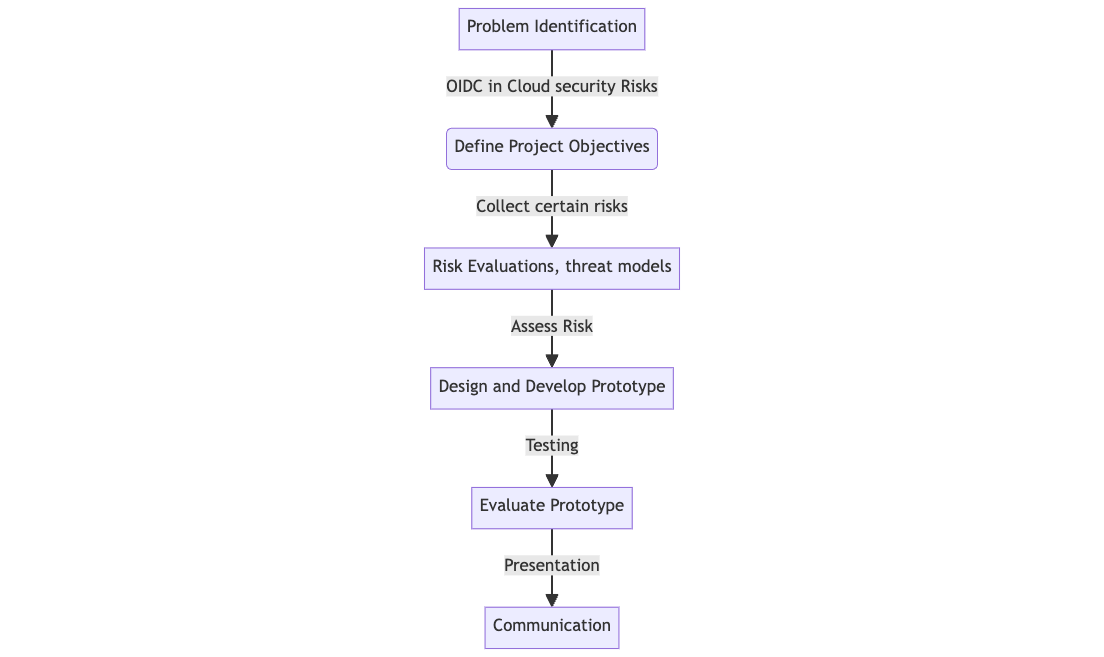
\includegraphics[width=\textwidth, height=320px]{pics/dsrm.png}
\end{figure}


\section{Thesis Outline}
